\documentclass{article}
\usepackage{amsmath}
\usepackage{natbib}
\usepackage{indentfirst}
\usepackage{graphicx}

\usepackage{listings}
\usepackage{color}
\definecolor{dkgreen}{rgb}{0,0.6,0}
\definecolor{gray}{rgb}{0.5,0.5,0.5}
\definecolor{mauve}{rgb}{0.58,0,0.82}
\lstset{frame=tb,
    language=Python,
    aboveskip=3mm,
    belowskip=3mm,
    showstringspaces=false,
    columns=flexible,
    basicstyle={\small\ttfamily},
    numbers=none,
    numberstyle=\tiny\color{gray},
    keywordstyle=\color{blue},
    commentstyle=\color{dkgreen},
    stringstyle=\color{mauve},
    breaklines=true,
    breakatwhitespace=true,
    tabsize=4
}

\title{Monte Carlo Course Group Project \\ 
Multilevel Monte Carlo Method in Pricing European Stock Exchange Option}
\author{Harold Kingsberg, Minh Tran, Peter Will}
\date{2017-05-15} 

\begin{document}
\maketitle
\tableofcontents

\newpage
\section{Introduction} 
	In this group project, we implement the Multilevel Monte Carlo (MLMC) method in path simulations in order to construct pricing of a European stock exchange option, under the assumptions of stochastic volatility in the Heston model, as outlined by \cite{heston93}. The MLMC method in path simulations was described by \cite{giles08}. The key advantage of this method is that for the same target level of accuracy (expressed in terms of confidence interval width, $\epsilon$), the MLMC method requires computing effort of $O(\epsilon^{-2}(log\epsilon)^2)$, compared to the standard Monte Carlo (MC) method which has computing cost of $O(\epsilon^{-3})$. 
    
    For the problem of our project, the stochastic volatility function prescribed by the Heston model does not satisfy the global Lipschitz condition, and thus the order of weak and strong convergence cannot be determined \cite{giles08} via theoretical methods.
	
	[xxx insert empirical results of the order of convergence]
	[TBD...summary about our results and cost savings]

\section{Heston Model and the European Exchange Option}
	Our project examines a European exchange option, which gives its owner the ability, but not the obligation, to exchange one unit of stock $S_2$ for one unit of stock $S_1$; this option can be exercised only at the specified expiry time T of the option. Thus the payoff of the option $P$ at time T is: $P(T)=max[0, S_1(T)-S_2(T)]$. The aim of our project is to employ Monte Carlo simulation to estimate the price of this European exchange option at time $t_0=0$ under the Heston stochastic volatility model.
    
    Before discussing the Heston model, we discuss the standard Black-Scholes assumptions, under which this exchange option can be priced using the Margrabe's formula given by \cite{margrabe78}. The Black-Scholes assumptions are that the stocks $S_1$ and $S_2$ have continuous dividend yield $q_1$ and $q_2$, respectively, and that their prices evolve based on the stochastic differential equation (SDE) with constant volatility as follows:
	\begin{align*}
	dS_1(t) &= \mu_1 S_1(t) dt + \sigma_1 S_1(t) dW_1(t) \\
	dS_2(t) &= \mu_2 S_2(t) dt + \sigma_2 S_2(t) dW_2(t)
	\end{align*}	
	
	In these equations, the two standard Brownian motions $W_1(t)$ and $W_2(t)$ are assumed to be correlated by a constant correlation coefficient $\rho$, satisfying $dW_1(t) \times dW_2(t) = \rho \times dt$. When the dynamics of the stocks are specified in the risk-neutral measure, the drift term $\mu_i$ is changed into $r-q_i$, where $r$ is the constant risk-free interest rate. Then the Margrabe's formula indicates that the value of the European exchange option at time $t_0=0$ is:
	\begin{align*}
	C(0) &= e^{-q_1 T} S_1(0) N(d_1) - e^{-q_2 T} S_2(0) N(d_2) \\
	d_1 &= \frac{ln(\frac{S_1(0)}{S_2(0)}) + (q_2 - q_1 + \frac{1}{2} \sigma^2) T}{\sigma \sqrt{T}} \\
	d_2 &= d_1 - \sigma \sqrt{T} \\
	\sigma &= \sqrt{\sigma_1^2 + \sigma_2^2 - 2 \rho \sigma_1 \sigma_2}
	\end{align*}	
	
	As we move from the Black-Scholes model to the Heston model, the key difference is that the volatility $\sigma$ associated with the diffusion term in the stock's SDE no longer remains a constant. Instead, in the Heston model, the square of the volatility (i.e. the variance) also follows a stochastic process characterized by an SDE. Hence, the dynamics of stock $S_i(t)$ in the Heston model consist of the equations as follows:
	\begin{align*}
	dS_i(t) &= \mu_i S_i(t) dt + \sqrt{\upsilon_i(t)} S_i(t) dW_i(t) \\
	d\upsilon_i(t) &= \kappa_i (\theta_i - \upsilon_i(t)) dt + \gamma \sqrt{\upsilon_i(t)} dZ_i(t) \\
	dW_i(t) \times dZ_i(t) &= \rho_i dt
	\end{align*}
	where $\kappa_i, \theta_i, \gamma_i$ are strictly positive constants, with $W_i(t)$ and $Z_i(t)$ being correlated one-dimensional Brownian motions.
    
	In this model, the variance $\upsilon_i(t)$ of the stock $S_i(t)$ follows a stochastic process with a mean-reverting characteristic. When $\upsilon_i(t)$ is higher than its mean-reverting level $\theta_i$, the drift term in the SDE of $\upsilon_i(t)$ becomes negative. The variance then has an underlying tendency to drift back to $\theta_i$. The opposite happens when the variance $\upsilon_i(t)$ is lower than its mean-reverting level $\theta_i$. Meanwhile, the constant parameter $\kappa_i$ influences the speed with which the variance reverts to $\theta_i$. 
	
	When we simulate the evolution of two stocks $S_1$ and $S_2$ in the Heston model, we will need to specify in advance the constant correlation coefficients for the Brownian motions in each of the stock's SDE and its associated variance's SDE. Specifically, we will need to specify the following symmetric positive definite correlation matrix for the four Brownian motions driving the diffusion terms:
	\begin{equation}
	corr
	\begin{bmatrix} 
	W_1  \\
	W_2  \\
	Z_1  \\
	Z_2  \\
	\end{bmatrix}
	=
	\begin{bmatrix} 
	1 & \rho(W_1,W_2) & \rho(W_1,Z_1) & \rho(W_1,Z_2) \\
	\rho(W_2,W_1) & 1 & \rho(W_2,Z_1) & \rho(W_2,Z_2) \\
	\rho(Z_1,W_1) & \rho(Z_1,W_2) & 1 & \rho(Z_1,Z_2) \\
	\rho(Z_2,W_1) & \rho(Z_2,W_2) & \rho(Z_2,Z_1) & 1 \\
	\end{bmatrix}
	\end{equation}
	
\section{Standard Monte Carlo for Euler-Maruyama Path Simulations}
	At the current time $t_0=0$, we are concerned with the payoff of an option with the expiry time $T$. We are interested in simulating the evolution of the stocks' prices over possible paths between the time $[0,T]$. The Euler-Maruyama method in path discretization starts with dividing this time interval $[0,T]$ into $K$ equispaced nodes of distance $h$ apart, where the notations include: $h = T/K$, $t_0=0$, $t_k=k \times h$. We start with $S_i(t_0)=S(0)$, and in order to simulate the stock price over one step from $S_i(t_k)$ to $S_i(t_{k+1})$ as well as to let its variance evolve under the Heston model, the full truncation method (\cite{andersen07}) indicates that:
	\begin{align}	
	S_i(t_{k+1}) - S_i(t_k) &= \mu_i S_i(t_k) h + \sqrt{\upsilon_i(t_k)^+} S_i(t_k) dW_i \\
	\upsilon_i(t_{k+1}) - \upsilon_i(t_k) &= \kappa_i (\theta_i - \upsilon_i(t_k)^+) h + \gamma \sqrt{\upsilon_i(t_k)^+} dZ_i(t) \\
	\upsilon_i(t_k)^+ &= max[\upsilon_i(t_k), 0]
	\end{align}
	where the increments of the Brownian motions, $dW_i$ and $dZ_i$, are sampled from correlated normal distributions with mean equal to 0, variance equal to the size of the incremental time step $h$, and correlations as specified in the correlation matrix (equation 1). 
	
	Under the Black-Scholes model, this path simulation simplifies to:
	\begin{equation}
	S_i(t_{k+1}) - S_i(t_k) &= \mu_i S_i(t_k) h + \sigma_i S_i(t_k) dW_i
	\end{equation}
	
	Using the above Euler-Maruyama path discretization, we can simulate one path travelled by the stock price(s) in the interval $[0,T]$, and calculate the payoff $P$ of an European option $P=C(T)$ based on the terminal stock prices $S_i(T)$ on this single path. For the vanilla European call option, this payoff will be $P(T)=max[S(t_K)-strike,0]$. For the European stock swap option, this payoff will be $P(T)=max[S_1(t_K)-S_2(t_K),0]$. We repeat the multi-step simulation in order to sample $N$ independent paths, and the average over these paths (after appropriate discounting) is an estimator of the price of the option at the current time $t_0=0$:
    \begin{equation}
    \widehat{C(0)} = D \times N^{-1} \times \sum_{i=1}^N P(\widehat{S(T)},T)
    \end{equation}
	where $D$ represents the discount factor. For example, when the stock dynamics are specified and simulated in the risk-neutral probability measure constant risk-free rate $r$, we have $D=e^{-rT}$.
    
    This method of repeatedly sampling $N$ independent paths represents the standard Monte Carlo method. According to \cite{giles08}, provided that the stock's drift and diffusion functions $\mu(\cdot)$ and $\sigma(\cdot)$, and the option's payoff function $P=P(S(T))$, satisfy certain conditions (including the global Lipschitz conditions), the estimator from the standard Monte Carlo method for Euler-Maruyama paths has an expected mean square error (MSE) that is asymptotically $O(N^{-1}) + O(h^2)$. 
    
	We can further examine the error by separating it into a discretization error and a statistical error. Closely following \cite{giles08}, we denote $P=P(S(T))$ as the payoff based on $S(T)$, whose expectation $E[P]$ is the quantity we are interested in estimating. In practice, we cannot simulate $S(T)$ and $P$, but instead rely on simulating small incremental time steps of size $h$ each. Let $\widehat{S(t)}$ be the approximation of $S(t)$ via simulating with time step $h$, and $\widehat{P_h}$ be the associated approximation of $P$, where the subscript $h$ is to emphasize the step size. Provided that conditions on $\mu(\cdot)$ and $\sigma(\cdot)$ are met, the orders of convergence of Euler-Maruyama are expressed as in \cite{higham15}:
	\begin{align*}
	\sup_{0 \leq t_k \leq T} (E[\widehat{S(t_k)}] - E[S(t_k)]) &= O(h) \\
	E[\sup_{0 \leq t_k \leq T}\mid \widehat{S(t_k)} - S(t_k)\mid ] &= O(h^{\frac{1}{2}})
	\end{align*}
    
	When we simulate $N$ independent paths, we are making an estimator of $E[\widehat{P}_h]$ instead of $E[P]$. Our estimator has a bias stemmed from the step size $h$, and the bias is $E[\widehat{P_h}] - E[P] = O(h)$, provided conditions are met (\cite{higham15}). This bias is a discretization error that is generally not influenced by $N$. Our second source of error is statistical and it depends on how many samples $N$ we generate to estimate $E[\widehat{P}_h]$. The statistical error is described by a confidence interval width $O(N^{-\frac{1}{2}})$, or variance $O(N^{-1})$.
	
    We target a certain level of accuracy expressed by $\epsilon$, the width of the confidence interval given by the Monte Carlo estimator. Specifying $\epsilon$ is equivalent to specifying a target standard deviation of the estimator as well as confidence level such as 90\% or 95\%. The MSE will then be $O(\epsilon^2)$. In order to achieve this level of accuracy via standard MC simulations, we will need the number of independent paths $N \sim O(\epsilon^{-2})$ and the step size $h \sim O(\epsilon)$. Given that on each single path the MC algorithm takes $T/h$ number of steps, the total computing effort from standard MC is $O(Nh^{-1})$, or $O(\epsilon^{-3})$. 
    
    For our group project, we implemented the following standard MC algorithm (for illustration and comparison with MLMC):
    \begin{lstlisting}
	target_std_error, confidence_level = get_user_input()
    if (user_provided_num_steps is None):
        num_steps_per_path = T / epsilon
    stat_tracker = new empty statistics tracker of simulated payoffs
    stat_tracker.assign(appropriate discount factor)
    while (std error given by stat_tracker > target_std_error):
        path = new simulated path
        payoff = calculate payoff(path)
        stat_tracker.add(payoff)
        update stat_tracker.mean, stat_tracker.stdev
    std_MC_estimator = stat_tracker.mean
    std_MC_sample_error = stat_tracker.stdev
    return std_MC_estimator, std_MC_sample_error
    \end{lstlisting}
    
    According to \cite{giles08}, the stochastic volatility function $\sigma(\cdot)$ under the Heston model does not satisfy the global Lipschitz condition, and as a result, there is no theoretical guarantee that with simulating the number of independent paths $N \sim O(\epsilon^{-2})$ and step size $h \sim O(\epsilon)$, the MSE will be $O(\epsilon^2)$. In our algorithm above, the number of paths $N$ is increased until the empirical standard error decreases below the targeted standard deviation. 
    
    [xxx we will graph to show results of N on yaxis and targeted stdev on xaxis, for Heston vanilla stock, to see if N is O(square)]	

\section{Multilevel Monte Carlo for Path Simulations}
	Developing on the standard Monte Carlo method above, the MLMC method for path simulations, when applied to Euler-Maruyama discretization, starts by simulating a high number of independent paths, whereby on each path, the step size is large. This represents the initial coarser levels of MLMC. The algorithm then proceeds to finer levels where there are fewer independent paths run on smaller step sizes. The overall MLMC estimator is the sum of the sample average from the coarsest level $l=0$, together with the refinements made from subsequent higher levels.
	
	Following notations from \cite{giles08}, let $\widehat{P_l}$ be the approximation of $P$ using \textit{one single path} only with the step size $h_l$ corresponding to the MLMC level $l$ (for $l=0,1,2,...L$, with $L$ being the finest level). We note that there is a bias as $E[\widehat{P_l}] \neq E[P]$, the difference between these quantities being the discretization error, or the bias from using $E[\widehat{P_l}]$ to approximate $E[P]$. In general, the discretization error of $E[\widehat{P_l}]$ depends most on the step size $h_l$ (instead of on the number of independent paths generated). Provided that  conditions on $\mu(\cdot)$, $\sigma(\cdot)$, and $P(\cdot)$ are met, then $E[\widehat{P_l} - P] = O(h_l)$ as $l\rightarrow \infty$. Our goal is to use $E[\widehat{P_L}]$ as the approximation (though biased) of $E[P]$, and thus we make an estimator of $E[\widehat{P_L}]$.
		
    The MLMC method does not directly estimate $E[\widehat{P_L}]$ using step size $h_L$ at the finest level. Instead it first writes $E[\widehat{P_L}] = E[\widehat{P_0}] + \sum_{l=1}^L E[\widehat{P_l} - \widehat{P_{l-1}}]$. The method then uses $N_l$ independent paths to make an estimator $\widehat{Y_l}$ for $Y_l = E[\widehat{P_l} - \widehat{P_{l-1}}]$. Also, the quantity $Y_0 = E[\widehat{P_0}]$ is estimated using $N_0$ paths, a fixed input (such as $N_0=10,000$). The overall MLMC estimator for $E[\widehat{P_L}]$ is then:
	$$\widehat{Y} = \sum_{l=0}^L \widehat{Y_l}$$
	
	Given that $E[\widehat{P_L}]$ is an approximation of $E[P]$ (though with a bias), MLMC uses $\widehat{Y}$ as an estimator for $E[P]$. Our task is to estimate the variance of this estimator $V[\widehat{Y}]$, as well as the highest level $L$ and the optimal $N_l$ to use at each level in order to meet a targeted accuracy $\epsilon$.
	
	We implemented two MLMC algorithms for this purpose. The first algorithm is detailed in \cite{giles15} and makes use of the following positive constants: $\alpha$ for the decay rate of the bias between $E[P_l]$ and $E[P]$; $\beta$ for the decay rate of $V_l$, the variance of the estimator $Y_l$; and $\gamma$ for the growth rate of the computing cost $C_l$ for the estimator $\widehat{Y_l}$ of $Y_l$ at level $l$. These constants are expressed in Theorem 1 of \cite{giles15} as follows:
	\begin{align*}
	\mid E[P_l -P] \mid &\leq c_1 2^{-\alpha l} \\
	V_l &\leq c_2 2^{-\beta l} \\
	C_l &\leq c_3 2^{\gamma l} \\
    \alpha &\geq \frac{1}{2} min(\beta, \gamma)
	\end{align*}
	
	The algorithm assumes existence and apriori knowledge of $\alpha, \beta, \gamma$. For each specific application (with different drift, diffusion, and payoff functions), the user can derive in advance the values of these constants using analysis theories. If these constants are not provided by the user, the algorithm attempts to estimate their values via OLS regressions. At each new level, with new estimated values for $E[P_l], V_l, C_l$, the regressions are run to update the estimated $\alpha, \beta, \gamma$. The first algorithm that we implemented from \cite{giles15} is as follows:
    
	\begin{lstlisting}
	target_std_error, confidence_level = get_user_input()
    epsilon = target_std_error * z_score(confidence_level)
	initial_N = 10000
    if alpha, beta, gamma are not provided by user:
        alpha, beta, gamma = 0, 0, 0
	
    # run at least L=0,1,2 levels 
    L = 2
    for each l inside [0,L]:
        generate initial_N paths
        on each path:
            walk the fine level to get one sample of payoff P(l)
            recombine steps from the fine level for the coarse level
            walk the coarse level to get one sample of payoff P(l-1)
        estimate m(l) = average of [P(l) - P(l-1)]
        estimate V(l) = variance of [P(l) - P(l-1)]
        estimate C(l) = computing cost in estimating E[P(l) - P(l-1)]
        expected_m_level = 2^(-alpha) * m(l-1)
        expected_v_level = 2^(-beta) * V(l-1)
        adjust m(l), V(l) so they are not lower than 0.5 * expected values
    
    if alpha, beta, gamma are not provided by user:
        estimate alpha by OLS with m(l)
        estimate beta by OLS with V(l)
        estimate gamma by OLS with C(l)
    
    for each level inside [0,L]:
        recalculate optimal_num_paths(l) per equation (3.1) Giles (2015)    
        if optimal_num_paths > current N(l):
            simulate more paths to update m(level), V(level), C(level)
    
    test for weak convergence using m(level) and alpha
    if not converged, L += 1 and repeat    
    \end{lstlisting}   
        
    A key point is that along one path, the same pseudo-random numbers are used to estimate $P_l$ and $P_{l-1}$. For example, if $M$ is the factor to refine a path at level $l$ to a coarser level $l-1$, then the step size along one path on level $l$ is $h_l  = M^{-l} \times T$, and we reconstitute $M$ adjacent steps at level $l$ to form one step at $l-1$. Along one path, we want to sample one value of $\widehat{P_l} - \widehat{P_{l-1}}$, and we repeatedly sample $N_l$ paths to estimate $Y_l = E[\widehat{P_l} - \widehat{P_{l-1}}]$, and $V_l = var(Y_l)$.
    
    The second algorithm we implemented is from section 5 of \cite{giles08} and does not require estimating $\alpha, \beta, \gamma$. Instead, the test for convergence in this algorithm is based on:
    $$\mid \widehat{Y}_L - M^{-1} \widehat{Y}_{L-1} \mid \leq \frac{1}{\sqrt{2}} (M^2 - 1) \epsilon$$
    
    The algorithm repeats increasing the highest level $L$ and re-estimating the optimal $N_l$ at all levels, coupled with running additional paths at each level if the updated $N_l$ is higher than what it had been previously. The process runs until the convergence condition is met.
    
    \begin{lstlisting}
	target_std_error, confidence_level = get_user_input()
    epsilon = target_std_error * z_score(confidence_level)
	initial_N = 10000
    
    L = 2
    for each l inside [0,L]:
        generate initial_N paths
        on each path:
            walk the fine level to get one sample of payoff P(l)
            recombine steps from the fine level for the coarse level
            walk the coarse level to get one sample of payoff P(l-1)
        estimate m(l) = average of [P(l) - P(l-1)]
        estimate V(l) = variance of [P(l) - P(l-1)]       
        
    for each level inside [0,L]:
        recalculate optimal_num_paths(l) per equation (12) Giles (2008)    
        if optimal_num_paths > current N(l):
            simulate more paths to update m(level), V(level), C(level)
    
    test for convergence
    
    if not converged, L += 1 and repeat    
    \end{lstlisting}
	
\section{Empirical Results}
    Our replication confirms the result of \cite{giles08} in the case of constant volatility stock. This demonstrates that MCMC's computing effort scales with $O(\epsilon^{-2})$ when the drift and diffusion functions of the stock satisfy the required conditions. 
    \begin{figure}
        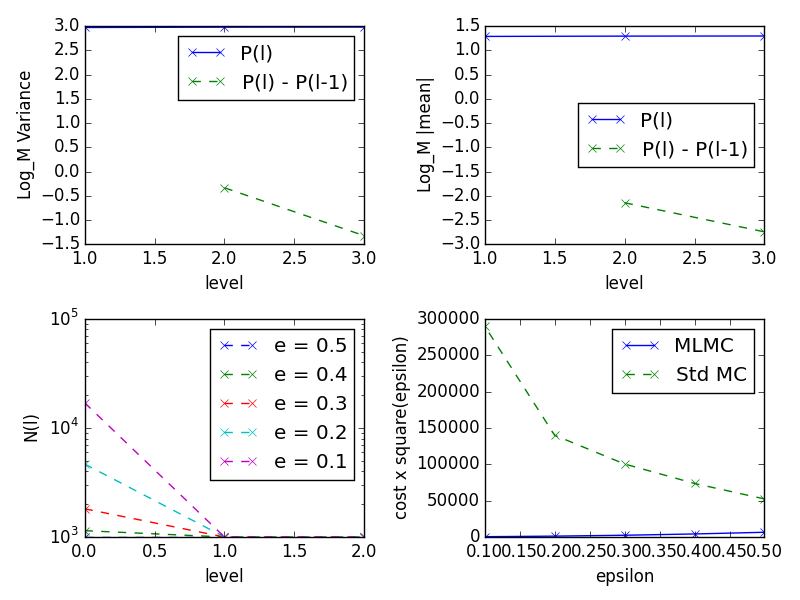
\includegraphics[width=\linewidth]{simple_layer_constvol_vanillacall.png}
        \caption{Scenario: European vanilla call on constant-vol stock}
        \label{fig:constvol_vanillacall}
    \end{figure}
    
    Figure \ref{fig:constvol_vanillacall} shows the most basic case where we price a vanilla European call option on a constant volatility stock. In the bottom right plot, cost $C$ is defined as the total number of steps taken. For standard MC, cost is $O(\epsilon^{-3})$ and thus for standard MC, $C \times \epsilon^{2}$ is a function of $O(\epsilon^{-1})$, which is the curve that we see. But MLMC in this case scales like $O(\epsilon^{-2})$ and thus for MLMC, $C \times \epsilon^{2}$ is much closer to a constant, which is why we see the straight line. 
    
    We now move to price the same vanilla European call but on a stock with Heston volatility. In this scenario, the diffusion of the stock no longer satisfies the required conditions. 
    \begin{figure}
        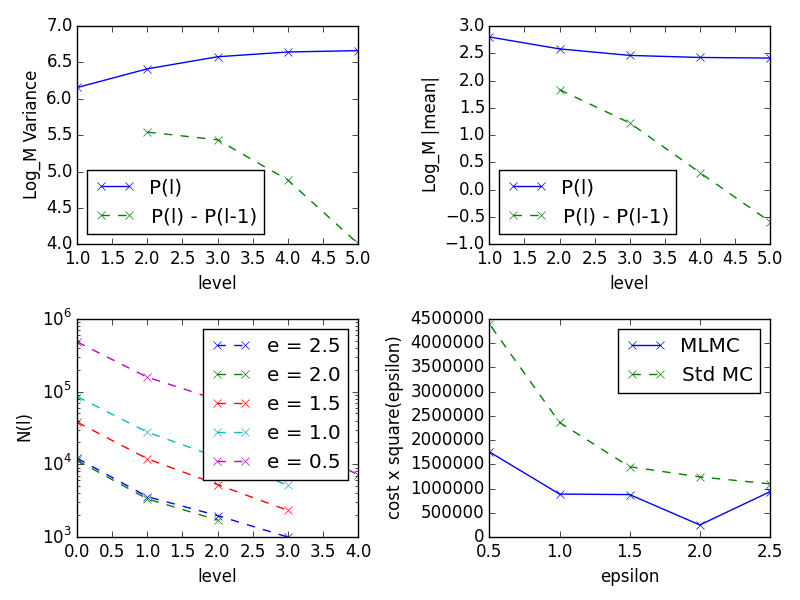
\includegraphics[width=\linewidth]{simple_layer_heston_vanillacall.png}
        \caption{Scenario: European vanilla call on Heston-vol stock}
        \label{fig:heston_vanillacall}
    \end{figure}
    
    We see from figure \ref{fig:heston_vanillacall} that our replication here still agrees with the figure from \cite{giles08} and MLMC still takes fewer total steps than standard MC. But in this case $C \times \epsilon^{2}$ is no longer close to a constant but more similar to a function of $\epsilon$. The scaling of MLMC as $\epsilon$ changes remains better than standard MC. 
    
    Our third scenario is a European stock exchange option on two stocks that have Heston volatility. 
    \begin{figure}
        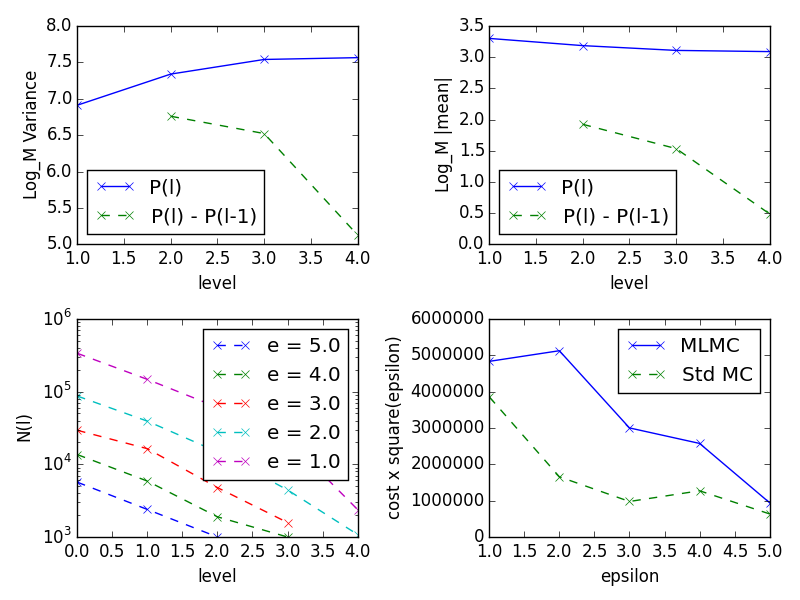
\includegraphics[width=\linewidth]{simple_layer_heston_swap.png}
        \caption{Scenario: European exchange option on two Heston-vol stocks}
        \label{fig:heston_swap}
    \end{figure}
    
    It is interesting to see here that our result changes compared to the previous two cases. MLMC is taking more steps than standard MC, and we cannot confirm that the computing effort of MLMC scales like $O(\epsilon^{-2})$. When the drift and diffusion of the stock no longer satisfy required conditions, the theorem from \cite{giles08} no longer guarantees that the computing effort of MLMC will be $O(\epsilon^{-2})$. In our example here, we cannot state whether MLMC scales in a similar way to standard MC, for the two Heston volatility stocks. This remains an area of further exploration.
    
\bibliography{group_project_mlmc_bibi}
\bibliographystyle{apalike}

\end{document}



















































